\chapter{Estado del arte} \label{chap:estadoarte}
\hrule
\vspace{3mm}

En este capítulo se hace un repaso de diferentes soluciones comerciales destinadas al soporte y posicionamiento de monitores, ordenadores o tablets. Dentro de todas las soluciones comerciales se centrará el estudio en las que están específicamente pensadas para su instalación en entornos médicos siempre que sea posible.
\\ 

Según el apoyo así como los tipos de grados de libertad hay diferentes configuraciones posibles, en este capítulo se verán algunos modelos concretos de cada caso evaluando sus características, ventajas e inconvenientes de los mismos de forma que se pueda generalizar a modelos equivalentes. De igual manera se podrán encontrar modelos motorizados y modelos sin motorizar, clasificación por la que serán agrupados a continuación.
\\ 

\section{Soportes articulados sin motorizar}

Dentro del grupo de soportes articulados sin motorizar se pueden clasificar según el tipo de anclaje que tienen, ya se enganchen al techo, pared, suelo, etc. 
\\

Dentro de cada tipo de anclaje los soportes comerciales disponibles son bastante parecidos por lo que se presentará un modelo concreto que encaje dentro de las dimensiones y capacidad de carga requeridas para la aplicación que se pretende explotar para sacar conclusiones generales sobre cada tipo de soporte.
\\ 
 
\subsection{Anclaje a la pared: Cotytech MW-M13P}

Dentro de esta gama (Cotytech MW-M*) se pueden encontrar modelos para soportar diferentes cargas. Concretamente se ha elegido el modelo con menores prestaciones y que soporta menos carga por ser suficiente para la aplicación que se pretende dar\footnote{Precios e información consultados en la página de compra online a 02 de Enero 2018 (\url{http://www.ergodirect.com/product_info.php?products_id=16881}) Precio a pasado a Euros según el cambio oficial en el día consultado.}. Otros modelos pueden incluir soporte para teclado, caja y cobertura para cables y enganche a pared, entre otros, suponiendo un incremento sobre el precio de este modelo.

\begin{minipage}{0.35\textwidth}
	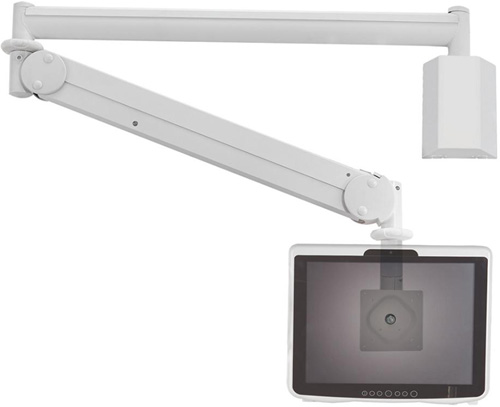
\includegraphics[width=\linewidth]{figuras/Imagenes_EstadoArte/Cotytech_MW-M13P.jpg}
\end{minipage}
\begin{minipage}{0.65\textwidth}\raggedright
	\hspace{1cm}
	\begin{itemize}
		\item Tipo de anclaje: Anclaje a la pared.
		\item Tipo de articulación: Articulaciones rotacionales.
		\item Capacidad de carga: entre $1kg$ y $6kg$.
		\item Extensión máxima: $185.7cm$.
		\item Número de grados de libertad: 5.
		\item Ángulos articulaciones: $370^o$ (brazo posición), $270^o$ (muñeca posición), $180^o$ (pared) $^1$. %fake footnote
		\item Ángulos de orientación: Tilt: $20^o$/- $35^o$ (muñeca orientación) and $20^o$/- $60^o$ (brazo orientación).
		\item Peso del soporte: $4.76 kg$.
		\item Precio estándar: 686.98\euro.
	\end{itemize}
\end{minipage}
\\

\begin{center}
\begin{minipage}{1\textwidth}
	\footnotesize{$^1$En la imagen se pueden ver tres puntos articulados diferenciados, el punto que se fija a la pared con un grado de libertad, el punto central del brazo, que tiene dos grados de libertad (se separarán entre orientación y posición, aunque su efecto no está desacoplado)y la muñeca, que incluye la articulación que se aprecia justo encima de la pantalla como la rotacional sobre la que queda enganchada la misma (con una clasificación análoga al caso intermedio).}
\end{minipage}
\end{center}
 
 Paralelamente a este modelo la marca Cotytech tiene, manteniendo el mismo esquema de mecánico, una versión que se podrá anclar al techo a un precio de 853.06\euro \footnote{Modelo Cotytech CM-M13 consultado el día 02 de Enero de 2018 en la página (\url{http://www.ergodirect.com/product_info.php?products_id=16891})}.
 \\ 
 
 
\subsection{Anclaje al techo: Titan Elite T2EQ-C8X5} 
 
 Concretamente se ha tomado el modelo con la montura doblada hacia arriba para un anclaje en el techo\footnote{Precios e información consultados en la página de compra online a 02 de Enero 2018 (\url{http://www.did-plus.com/en/medical-arms/articulated-monitor-mounts.html}). Precio a pasado a Euros según el cambio oficial en el día consultado.} (hay opción de adquirirlo con la tubería del extremo a anclar doblada hacia abajo para anclarlo en la pared).
 
 \begin{minipage}{0.35\textwidth}
 	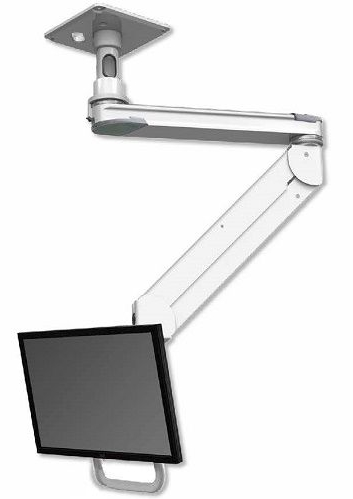
\includegraphics[width=\linewidth]{figuras/Imagenes_EstadoArte/T2EQ.jpg}
 \end{minipage}
 \begin{minipage}{0.65\textwidth}\raggedright
 	\hspace{1cm}
 	\begin{itemize}
 		\item Tipo de anclaje: Anclaje al techo.
 		\item Tipo de articulación: Articulaciones rotacionales.
 		\item Capacidad de carga: hasta $12.7kg$ en diferentes configuraciones.
 		\item Extensión máxima: $106cm$ (la longitud vertical del anclaje al techo variará según se elija al comprar).
 		\item Número de grados de libertad: 5.
 		\item Ángulos articulaciones: $360^o$ para las tres primeras articulaciones que rotan sobre el eje horizontal.
 		\item Ángulos de orientación: Tilt: $50^o$.
 		 		\item Peso del soporte: $9kg$.
 		\item Precio estándar: 628.30\euro.
 	\end{itemize}
 \end{minipage}
 \\ 
 
 Este mismo modelo cuenta con diferentes enganches y longitudes de los tubos que permiten anclarlo al suelo, al techo o a la pared indistintamente.
 \\ 
 
 
\subsection{Anclaje a una mesa o superficie de trabajo: Ergotron LX Sit-Stand Desk Arm} 
 
%https://www.ergotron.com/en-us/products/product-details/45-360#/
 
 De entre la gama incluida en los modelos de Ergotron LX se ha elegido aquel que tenía unas dimensiones más ajustadas a las necesidades reales\footnote{Precios e información consultados en la página de compra online a 02 de Enero 2018 (\url{https://www.ergotron.com/en-us/products/product-details/45-360\#/}).}. En general el resto de la gama y otros soportes similares tienen unas dimensiones más reducidas.
 
 \begin{minipage}{0.35\textwidth}
 	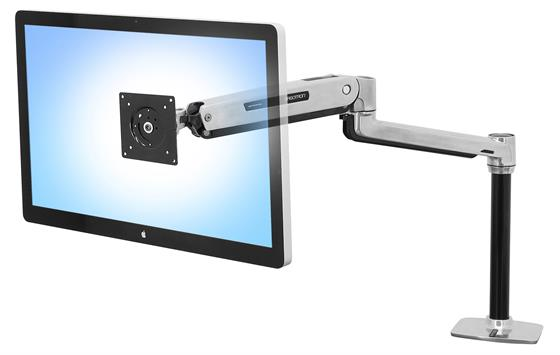
\includegraphics[width=\linewidth]{figuras/Imagenes_EstadoArte/LX_Sit-Stand_Desk_Arm.jpg}
 	\\ 
 	
 	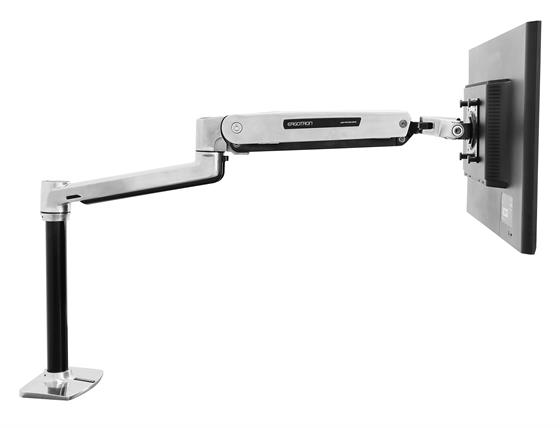
\includegraphics[width=\linewidth]{figuras/Imagenes_EstadoArte/LX_Sit-Stand_Desk_Arm_2.jpg}
 \end{minipage}
 \begin{minipage}{0.65\textwidth}\raggedright
 	\hspace{1cm}
 	\begin{itemize}
 		\item Tipo de anclaje: Anclaje a una mesa, camilla o similar.
 		\item Tipo de articulación: Primera articulación prismática, resto rotacionales.
 		\item Capacidad de carga: hasta $11.3kg$.
 		\item Extensión máxima: se puede variar hasta $36cm$ en altura (articulación prismática, esta es susceptible de ser modificada para ajustarla a otras alturas) y alcanza una extensión de $84cm$
 		\item Número de grados de libertad: 6 (una prismática y cinco rotacionales).
 		\item Ángulos articulaciones: $180^o$ la primera articulación, fija al anclaje; $360^o$ a mitad del brazo y $180^o$ en la muñeca.
 		\item Ángulos de orientación: Tilt: (giro sobre el eje medio horizontal de la pantalla) $75^o$; Pan (eje perpendicular a la pantalla): $360^o$.
 		\item Peso del soporte: $8.9kg$.
 		\item Precio estándar: 247.00\euro – 299.00\euro dependiendo de la tienda y configuración.
 	\end{itemize}
 \end{minipage}
 \\ 
 
 \vspace{0.1cm} 
 Este mismo modelo cuenta con diferentes enganches y longitudes de los tubos que permiten anclarlo al suelo, al techo o a la pared indistintamente.
 
 \subsection{Consideraciones generales}

\section{Soportes articulados motorizados}
 \subsection{Consideraciones generales}
 
\section{Brazos robóticos para asistencia de pacientes} 

	En general para el propósito que se plantea en este proyecto se podría adaptar una solución robótica comercial implementando una interfaz entre la tablet y el controlador del brazo. En esta sección se presentan algunos modelos de brazos robóticos especialmente pensados como robots asistenciales, preparados para una interacción directa con pacientes en entornos hospitalarios o caseros \completarCon{not the word...}.
	
 \subsection{JACO 3 fingers, Kinova robotics}
	 Pertenece a la línea de productos de Kinova robotics especialmente diseñados como robots asistenciales. Están pensados para una interacción directa con el paciente o usuario de forma que pueda convertirse en una extensión del mismo proporcionándole una mayor independencia. \footnote{ Información consultada en la página de la compañía a 20 de Enero 2018 (\url{http://www.kinovarobotics.com/assistive-robotics/products/robot-arms/})}
	 \\ 
	 
	 Este modelo, Jaco viene en dos formatos, con tres y con dos dedos en el manipulador. 
	  
	  \begin{minipage}{0.35\textwidth}
	  	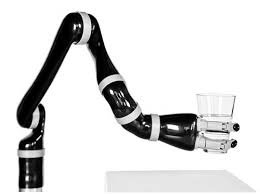
\includegraphics[width=\linewidth]{figuras/Imagenes_EstadoArte/jaco-3-finger.jpg}
	  \end{minipage}
	  \begin{minipage}{0.65\textwidth}\raggedright
	  	\hspace{1cm}
	  	\begin{itemize}
	  		\item Tipo de anclaje: Adaptativo a una mesa, silla de ruedas, etc
	  		\item Tipo de articulación: 6 grados de libertad rotacionales
	  		\item Capacidad de carga: entre $1.8kg$ y $1.6kg$ dependiendo de la versión elegida (con tres dedos tiene una capacidad menor).
	  		\item Extensión máxima: alcanza $90cm$.
	  		\item Número de grados de libertad: 6.
	  		\item Ángulos de posición: Unlimited joint rotations \completarCon{¿?¿?}
	  		\item Ángulos de orientación: $55^o$ en la muñeca.
	  		\item Peso del brazo: $5.7kg$.
	  		\item Precio estándar: desde 34900\euro.
	  	\end{itemize}
	  \end{minipage}
	  \\ 
	  
	  \vspace{0.1cm} 
	  De esta marca se puede adquirir también el modelo MICO con algo menos de alcance ($70cm$). Los grados de libertad ofertados varían entre 4 y 7, se ha optado por tomar una solución simular a la requerida.
	 
 \subsection{Consideraciones generales}